% B.Tech. Project: Part A presentation (Beamer)
% Build:  cd presentation && latexmk -pdf part_a_final.tex
%   or:   pdflatex part_a_final && pdflatex part_a_final
% Figures are read directly from the repository result folders (see \graphicspath).
\documentclass[aspectratio=169,11pt,xcolor=table]{beamer}

\usetheme{Madrid}
\usecolortheme{default}
\usefonttheme{professionalfonts}

\usepackage[T1]{fontenc}
\usepackage{lmodern}
\usepackage{amsmath,amssymb}
\usepackage{booktabs}
\usepackage{array}
\usepackage{tikz}
\usetikzlibrary{arrows.meta,positioning,shapes.geometric,calc}
\usepackage{graphicx}
\usepackage{listings}

\graphicspath{%
  {../results/figures/}%
  {../results/v2/}%
}

% ---------- colours ----------
\definecolor{iitblue}{RGB}{16,52,110}
\definecolor{accent}{RGB}{200,40,40}
\definecolor{good}{RGB}{20,120,60}
\definecolor{soft}{RGB}{235,240,248}
\setbeamercolor{structure}{fg=iitblue}
\setbeamercolor{palette primary}{bg=iitblue,fg=white}
\setbeamercolor{palette secondary}{bg=iitblue!85!black,fg=white}
\setbeamercolor{palette tertiary}{bg=iitblue!70!black,fg=white}
\setbeamercolor{frametitle}{bg=iitblue,fg=white}
\setbeamercolor{title}{bg=iitblue,fg=white}
\setbeamercolor{block title}{bg=iitblue,fg=white}
\setbeamercolor{block body}{bg=soft}
\setbeamercolor{block title alerted}{bg=accent,fg=white}
\setbeamercolor{block body alerted}{bg=accent!8}
\setbeamercolor{block title example}{bg=good,fg=white}
\setbeamercolor{block body example}{bg=good!8}
\setbeamertemplate{navigation symbols}{}
\setbeamertemplate{itemize items}[circle]
\setbeamertemplate{blocks}[rounded][shadow=false]
\setbeamerfont{frametitle}{size=\large,series=\bfseries}

\newcommand{\hl}[1]{\textcolor{accent}{\textbf{#1}}}
\newcommand{\gd}[1]{\textcolor{good}{\textbf{#1}}}
\newcommand{\best}[1]{\textbf{\textcolor{good}{#1}}}
\newcommand{\ours}{\rowcolor{good!15}}
\newcommand{\takeaway}[1]{%
  \vfill
  \begin{alertblock}{}\centering\textbf{#1}\end{alertblock}}

\lstset{basicstyle=\ttfamily\scriptsize,backgroundcolor=\color{black!85},
  basicstyle=\ttfamily\scriptsize\color{white},keywordstyle=\color{cyan!70},
  commentstyle=\color{green!60},language=C,columns=fullflexible,
  frame=none,xleftmargin=4pt,xrightmargin=4pt,aboveskip=0pt,belowskip=0pt}

\AtBeginSection[]{%
  \begin{frame}[noframenumbering]{Outline}
    \tableofcontents[currentsection,hideallsubsections]
  \end{frame}
}

% ---------- title ----------
\title[Part A: Lighter Fronthaul, Faster DU]{Part A: Making the Fronthaul Lighter and the DU Faster}
\subtitle{Structure-aware IQ compression, RMT-guided warm-start complex inversion,\\
and a fused C/AVX-512 RZF precoder kernel for O-RAN 7-2x}
\author[M.~Yadav \& H.~Choudhary]{Mayank Yadav \and Harshvardhan Choudhary}
\institute[B.Tech. Project]{B.Tech. Project --- Final Evaluation}
\date{November 2026}

\begin{document}

\begin{frame}
  \titlepage
\end{frame}

\begin{frame}{Outline}
  \tableofcontents[hideallsubsections]
\end{frame}

% =====================================================================
\section{Motivation and Contributions}

\begin{frame}{Why Part A? Two bottlenecks of a 5G/6G O-RAN cell}
  \begin{columns}[T]
    \begin{column}{0.48\textwidth}
      \begin{block}{1. The fronthaul is huge}
        \begin{itemize}
          \item Raw 64-antenna cell: $\approx 15.4$ Gbit/s
          \item DU-side precoding, 100 MHz, 64 streams: \hl{118 Gbit/s}
          \item O-RAN BFP only shortens numbers: $\approx 4\times$
        \end{itemize}
        $\Rightarrow$ compression that exploits channel structure
      \end{block}
    \end{column}
    \begin{column}{0.48\textwidth}
      \begin{block}{2. The DU has 0.5 ms per slot}
        \begin{itemize}
          \item RZF per PRB: $G = HH^H + \alpha I$, \; $W = H^H G^{-1}$
          \item 273 PRBs $\times$ complex $K\times K$ inverse every slot
          \item numpy + LAPACK: \hl{3.2 ms} for $K=16$ (6$\times$ over budget)
        \end{itemize}
        $\Rightarrow$ fast, accurate complex inversion
      \end{block}
    \end{column}
  \end{columns}
  \vspace{4mm}
  \centering
  \textbf{Our answer:} compress the data with its own structure, and invert the complex
  channel matrices with an RMT-guided method running on hand-optimised kernels.
  \takeaway{Part A attacks both bottlenecks: fewer bits on the link, and a precoder that fits in the slot.}
\end{frame}

\begin{frame}{Our Part A contributions at a glance}
  \begin{columns}[T]
    \begin{column}{0.32\textwidth}
      \begin{block}{CSEE \& RAS-BFP}
        \gd{13--16$\times$} compression vs $\approx 4\times$ for O-RAN BFP;
        3--6$\times$ faster than SVD
      \end{block}
      \begin{exampleblock}{Warm-start tracking}
        \gd{2.7$\times$} fewer GEMMs, \gd{30$\times$} lower loss at pedestrian speed;
        never diverges at 120 km/h
      \end{exampleblock}
    \end{column}
    \begin{column}{0.32\textwidth}
      \begin{exampleblock}{ACAFS}
        Rank-adaptive functional split: \gd{55--75\,\%} bandwidth cut at high SNR
      \end{exampleblock}
      \begin{block}{Fused C/AVX-512 kernel}
        Whole RZF precoder \gd{10--15$\times$} faster than numpy+LAPACK; fits the 0.5 ms slot
      \end{block}
    \end{column}
    \begin{column}{0.32\textwidth}
      \begin{block}{RMT-WS inversion}
        Complex Hermitian Grams: \gd{6 GEMMs} vs $>10$ for Neumann-type methods
      \end{block}
      \begin{exampleblock}{RU-side precoding}
        \gd{$-72\,\%$} fronthaul at 99.7\,\% of exact RZF sum-rate
      \end{exampleblock}
    \end{column}
  \end{columns}
  \takeaway{From compression theory to a slot-feasible precoder: a complete DU-side toolchain.}
\end{frame}

% =====================================================================
\section{IQ Compression and Adaptive Split}

\begin{frame}{Structure-aware IQ compression}
  \centering
  $Y = H \odot X + W \in \mathbb{C}^{M\times N}$, \quad $M=64$ antennas, $N=1200$ subcarriers, 3GPP TDL-A
  \vspace{2mm}
  \begin{columns}[T]
    \begin{column}{0.48\textwidth}
      \begin{block}{CSEE --- delay-domain sparse encoder}
        \begin{enumerate}
          \item IFFT along subcarriers $\to$ delay domain
          \item Keep top-$K$ taps (channel is sparse in delay)
          \item Per-antenna BFP; FFT back at the receiver
        \end{enumerate}
        \textbf{Theorem 1:}
        $\mathrm{NMSE} \le \dfrac{\sigma^2_{\mathrm{tail}}}{\sigma^2_Y} + \dfrac{\Delta^2}{12}\dfrac{K}{MN\sigma_Y^2}$\\[1mm]
        Complexity $O(MN\log N)$
      \end{block}
    \end{column}
    \begin{column}{0.48\textwidth}
      \begin{exampleblock}{RAS-BFP --- randomised sketch + QR}
        \begin{enumerate}
          \item SRHT sketch $Z = \Omega Y \in \mathbb{C}^{r\times N}$
          \item Thin QR $Z^H = QR$; project $L = YQ$
          \item Send BFP$(L)$, BFP$(Q)$; \; $Y \approx LQ^H$
        \end{enumerate}
        \textbf{Theorem 2:} $\|Y - LQ^H\|_F^2 \le (1+\varepsilon_r)\|Y - Y_r\|_F^2$ w.h.p.\\
        \textbf{Theorem 4:} $r^\star = \big\lfloor \sqrt{B_{\mathrm{total}}/(b(M+N))} \big\rceil$, \; $O(rMN)$
      \end{exampleblock}
    \end{column}
  \end{columns}
  \takeaway{Both encoders come with provable error bounds and lower complexity than SVD.}
\end{frame}

\begin{frame}{Compression: 4$\times$ more than the O-RAN standard}
  \begin{columns}[c]
    \begin{column}{0.46\textwidth}
      \small $M=64$, $N=1200$, SNR 20 dB, TDL-A\\[2mm]
      \footnotesize\setlength{\tabcolsep}{4pt}
      \begin{tabular}{lcc}
        \toprule
        Method & Compression & Encode \\
        \midrule
        O-RAN BFP ($b=8$) & 3.9$\times$ & 3.1 ms \\
        Truncated SVD ($r=12$) & 16.2$\times$ & 18--30 ms \\
        \ours CSEE (ours) & \best{12.7$\times$} & \best{5.2 ms} \\
        \ours RAS-BFP (ours) & \best{16.2$\times$} & \best{7.2 ms} \\
        \bottomrule
      \end{tabular}
      \vspace{3mm}
      \begin{itemize}\footnotesize
        \item 13--16$\times$ compression at $\approx -20$ dB NMSE
        \item RAS-BFP: SVD-level compression, 3--4$\times$ faster
        \item CSEE: 4--6$\times$ faster than SVD; $\approx 63\times$ at the $K=60$ knee
        \item Stable NMSE across SNR $-5$ to 30 dB
      \end{itemize}
    \end{column}
    \begin{column}{0.5\textwidth}
      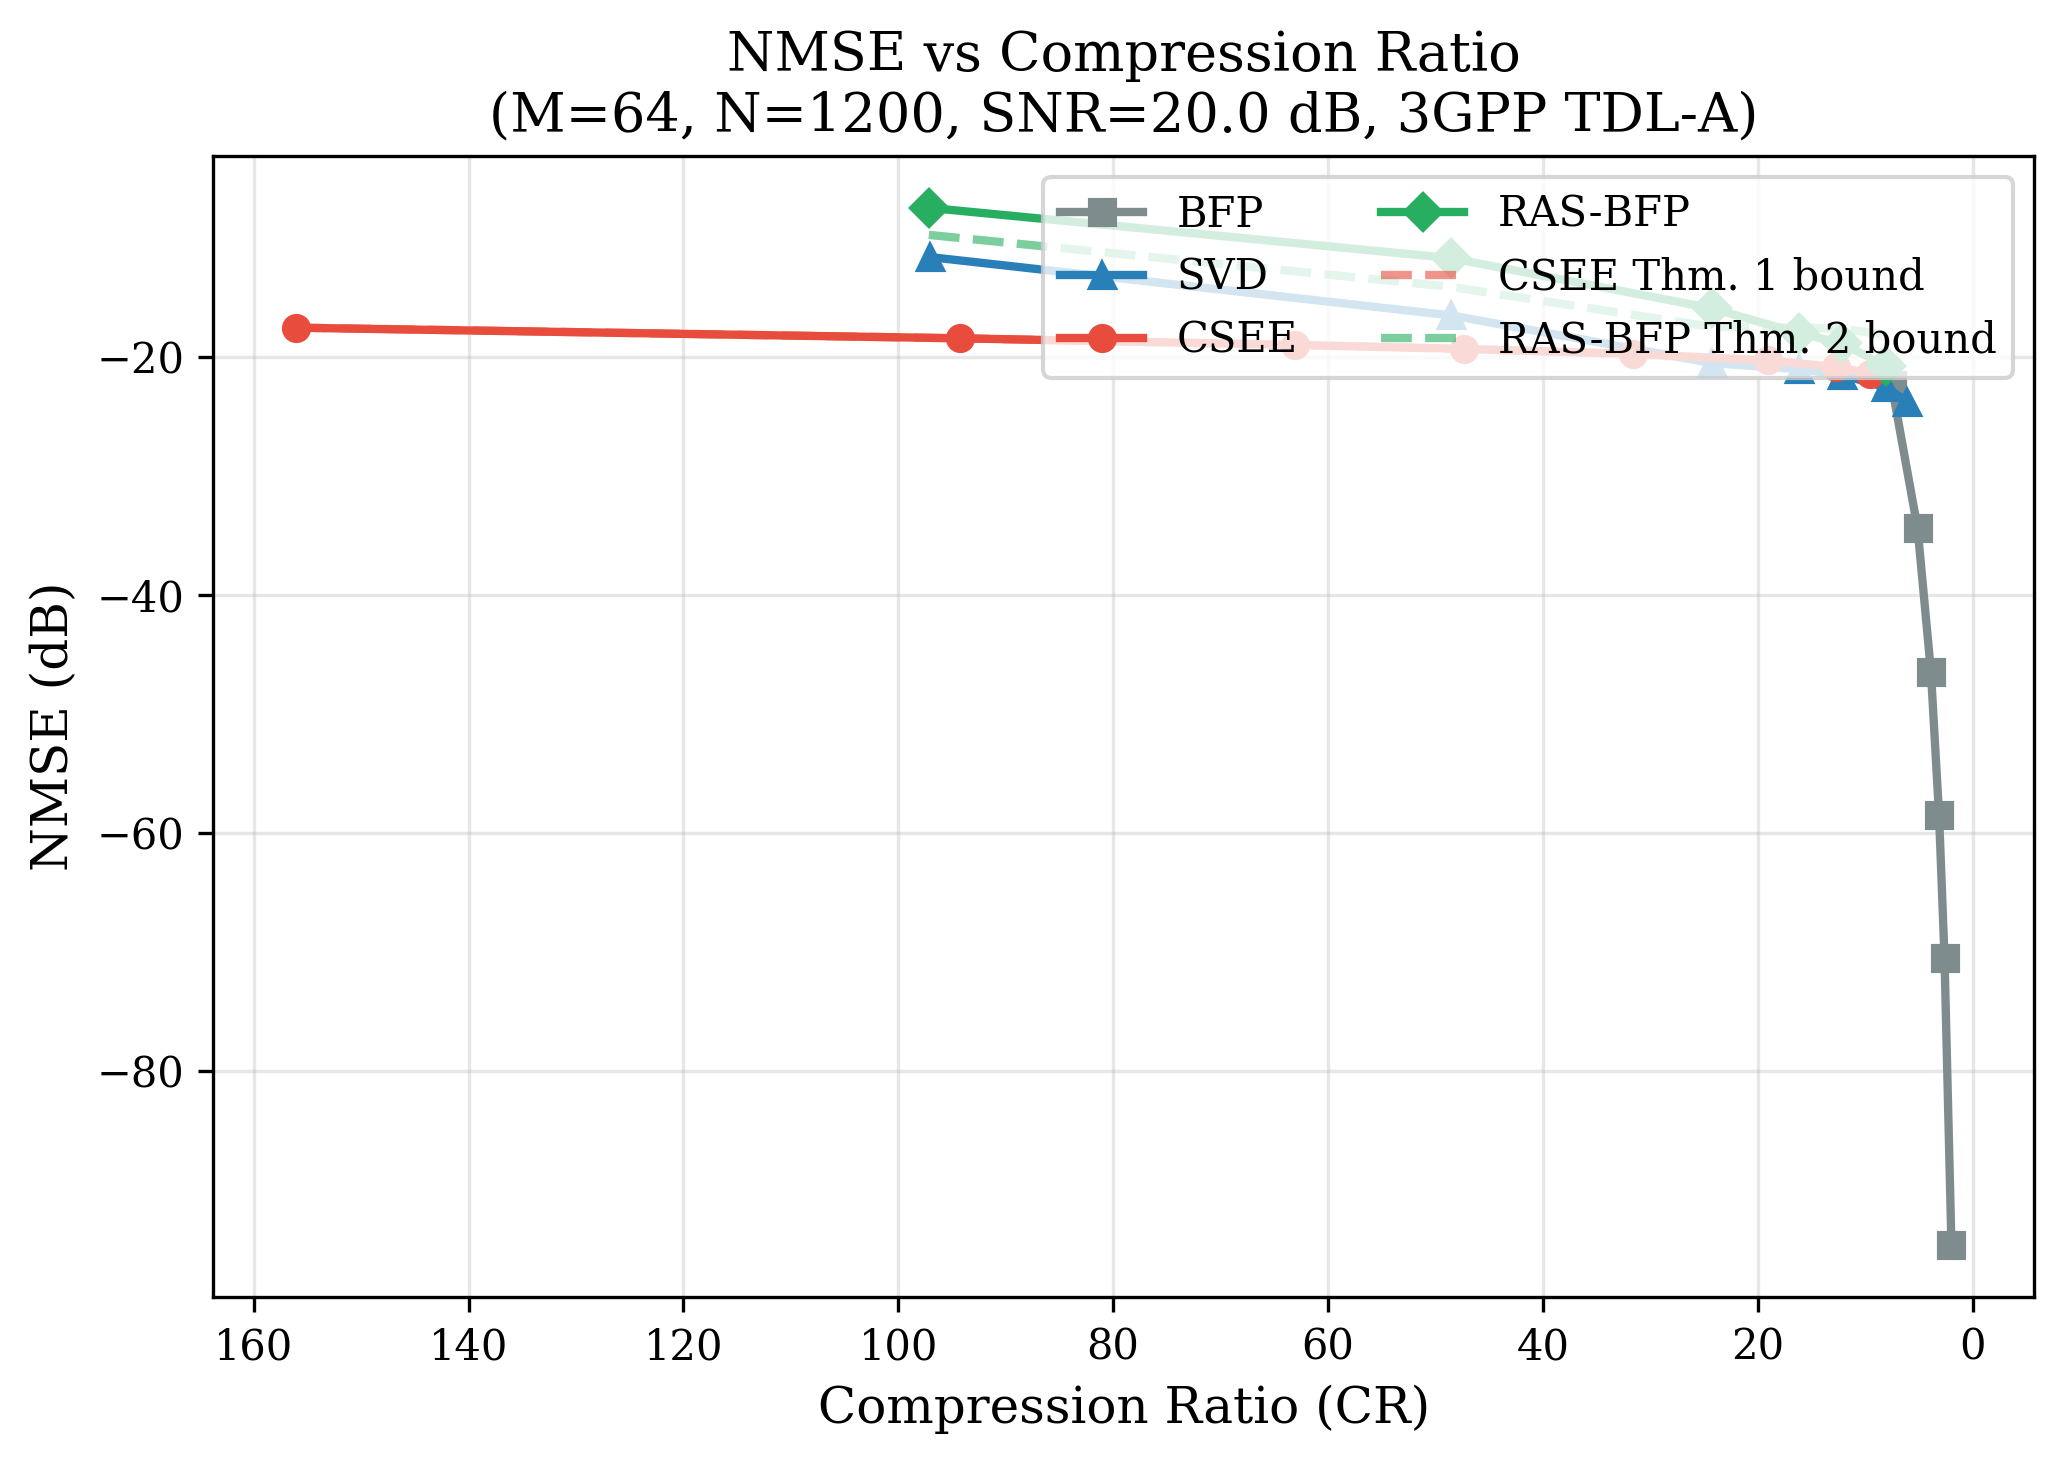
\includegraphics[width=\linewidth]{exp1_nmse_vs_cr.png}
    \end{column}
  \end{columns}
  \takeaway{RAS-BFP matches SVD compression at a fraction of its encode time.}
\end{frame}

\begin{frame}{ACAFS: rank-adaptive functional split}
  \begin{columns}[c]
    \begin{column}{0.42\textwidth}
      \small Per-UE rank fraction $r/M$ picks the O-RAN split:\\[1mm]
      \centering\footnotesize
      \begin{tabular}{cc}
        \toprule
        Rank fraction $r/M$ & Split \\
        \midrule
        $< 0.15$ & 7.2x \\
        $0.15$ -- $0.55$ & 7.1 \\
        $\ge 0.55$ & 6 \\
        \bottomrule
      \end{tabular}
      \raggedright
      \begin{itemize}\footnotesize
        \item \textbf{Theorem 5:} closed-form bandwidth saving vs a fixed Split 6
        \item $\approx 33\,\%$ saving for uniformly spread ranks
        \item \gd{55--75\,\%} saving at high SNR (rank collapse)
        \item Decision per UE, from the rank the encoder already computes
      \end{itemize}
    \end{column}
    \begin{column}{0.56\textwidth}
      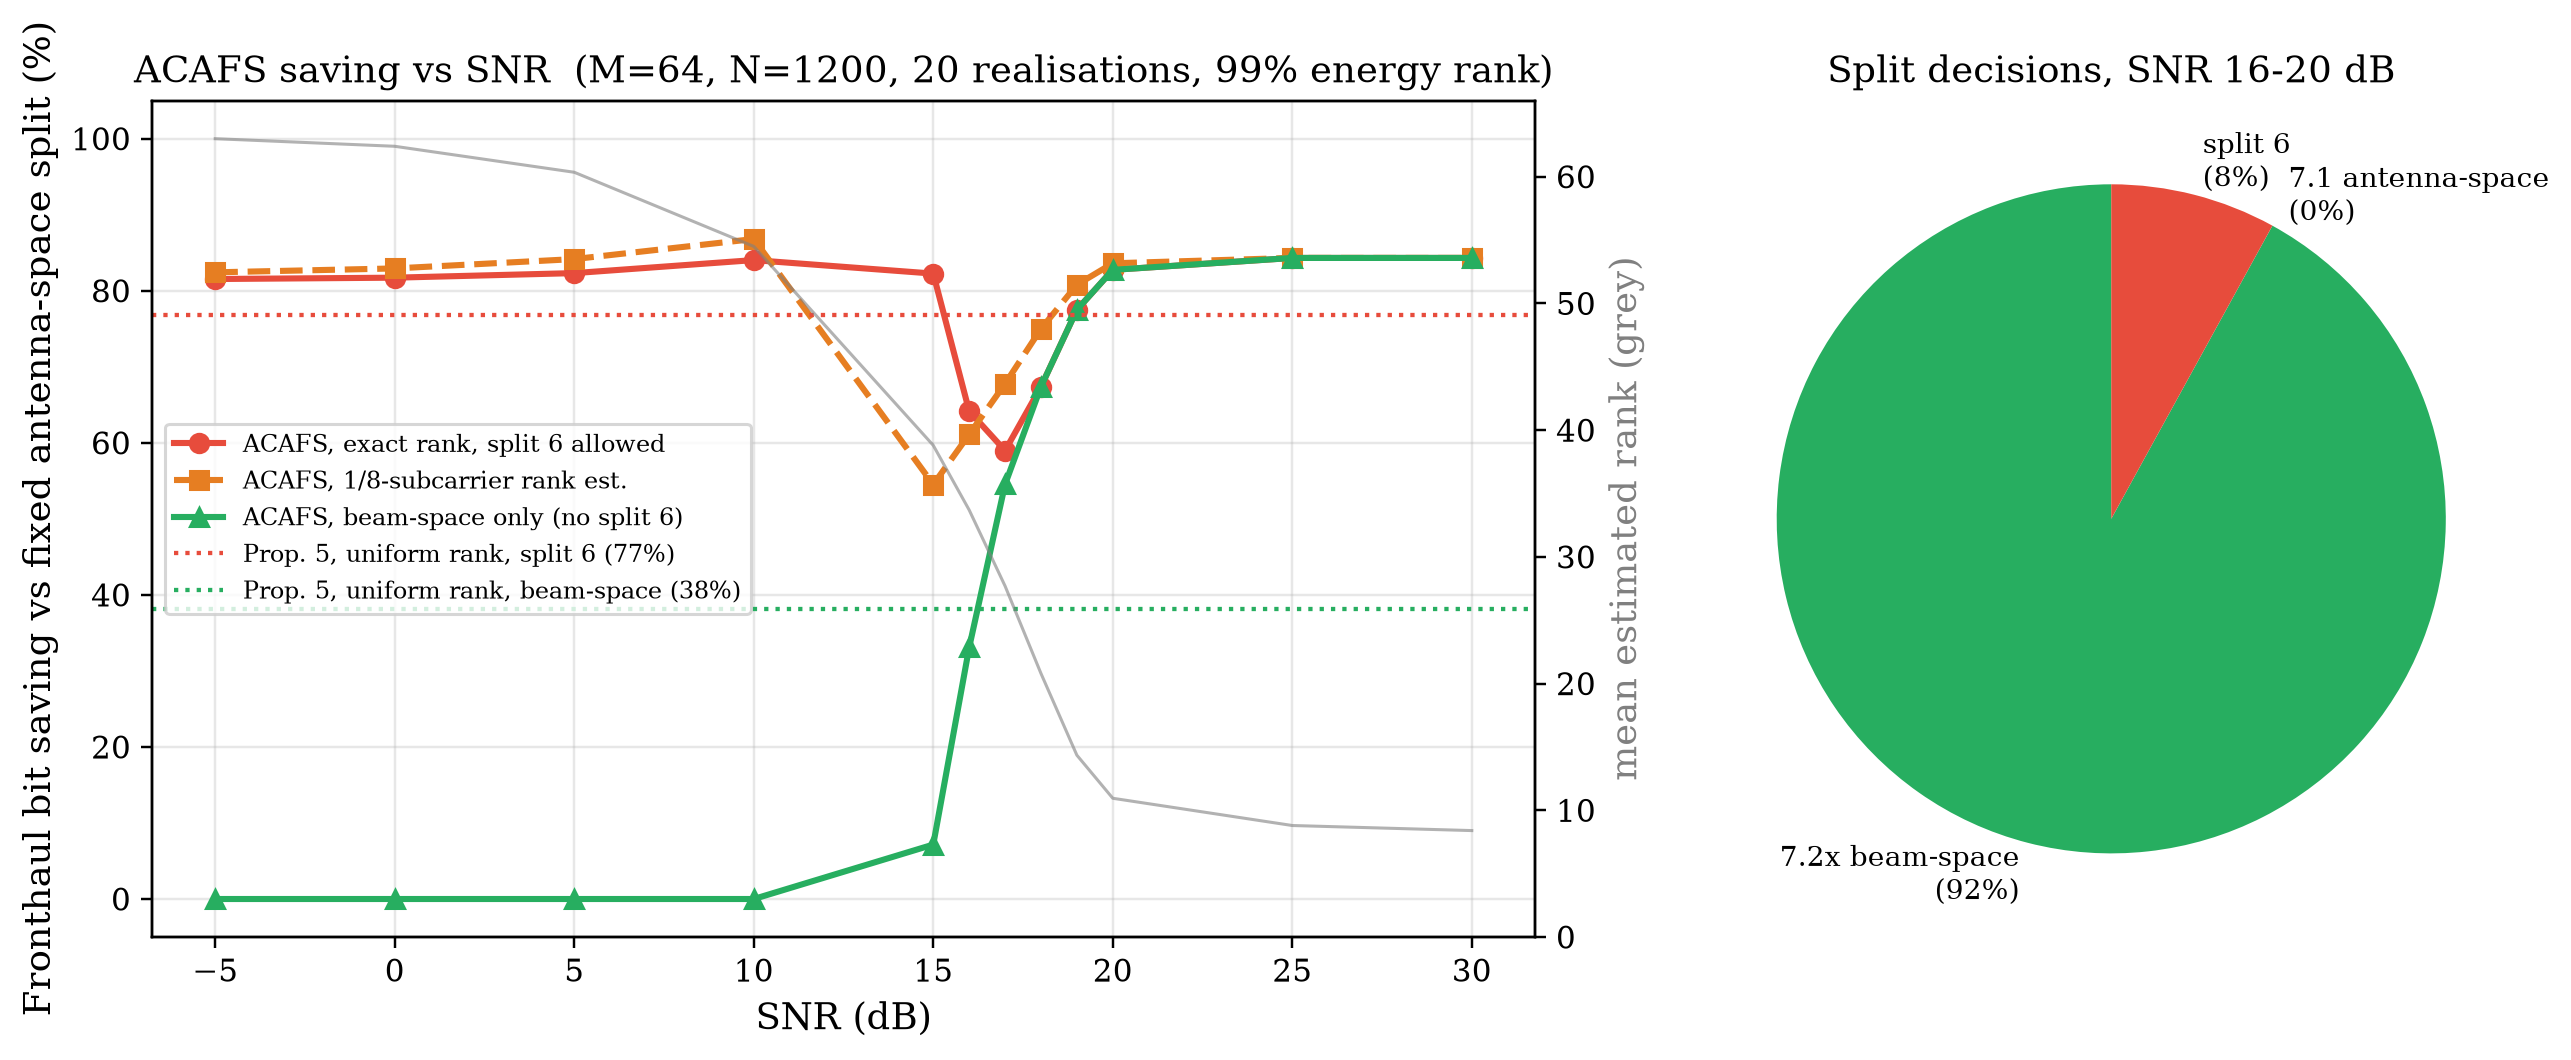
\includegraphics[width=\linewidth]{exp3_acafs.png}
    \end{column}
  \end{columns}
  \takeaway{The split adapts to the channel instead of being fixed at deployment.}
\end{frame}

% =====================================================================
\section{RMT-WS: Complex Matrix Inversion}

\begin{frame}{The real DU workload: complex RZF precoding}
  \begin{columns}[T]
    \begin{column}{0.5\textwidth}
      \begin{block}{Realistic complex channels (\texttt{cmatinv/})}
        \begin{itemize}\small
          \item 3GPP TR 38.901 UMa NLOS path loss + shadowing (near-far)
          \item TDL-A 23-tap profile over 100 MHz
          \item Per-user angular-spread spatial correlation
          \item Rician line-of-sight option
          \item Clarke/Jakes aging $\rho = J_0(2\pi f_D T)$: 3--120 km/h
          \item $M = 64/128$, $K = 8/16/32$, 273 PRBs, 30 kHz, 3.5 GHz
        \end{itemize}
      \end{block}
    \end{column}
    \begin{column}{0.46\textwidth}
      \begin{exampleblock}{Per PRB, every 0.5 ms slot}
        \[
          G = HH^H + \alpha I \in \mathbb{C}^{K\times K}
        \]
        \vspace{-2mm}\centering (complex Hermitian)
        \[
          W = H^H G^{-1} \in \mathbb{C}^{M\times K}
        \]
        \centering $\times$ 273 PRBs inside one slot
      \end{exampleblock}
      \textbf{Our question:} can the whole complex precoder run inside the slot on a CPU DU,
      and can inversion exploit the channel's statistics?
    \end{column}
  \end{columns}
\end{frame}

\begin{frame}{RMT-WS: random-matrix-guided warm-start inversion}
  \begin{columns}[T]
    \begin{column}{0.6\textwidth}
      \begin{enumerate}\small
        \item \textbf{Equilibrate} $\hat G = D^{-1/2} G D^{-1/2}$ --- removes the near-far spread
        \item \textbf{Eigensolve-free spectral interval} (Marchenko--Pastur + moment match):
          \[ v = \|\hat G\|_F^2/K - 1, \qquad [a,b] = 1 + v/\bar s \mp 2\sqrt{v} \quad (K^2 \text{ work}) \]
        \item \textbf{Cold start:} Chebyshev polynomial on $[a,b]$, then Newton--Schulz
          $X \leftarrow X(2I - \hat G X)$ (quadratic, pure GEMMs)
        \item \textbf{Tracking:} next slot starts from the previous inverse
        \item \textbf{Residual certificate} $\|(I - \hat G X)z\|/\|z\|$ picks the Newton steps
          per PRB, or falls back to a cold start --- always safe
      \end{enumerate}
    \end{column}
    \begin{column}{0.36\textwidth}
      \begin{exampleblock}{Why it fits the DU}
        \begin{itemize}\small
          \item[\checkmark] Adapts to correlated and near-far channels automatically
          \item[\checkmark] No eigen-decomposition
          \item[\checkmark] Only matrix multiplies: GPU / NPU / tensor-core friendly
          \item[\checkmark] Cost adapts to user speed
          \item[\checkmark] Built-in accuracy certificate
        \end{itemize}
      \end{exampleblock}
    \end{column}
  \end{columns}
  \takeaway{Random-matrix theory gives the inverse a head start; the certificate keeps it safe.}
\end{frame}

\begin{frame}{Cold-start inversion: fewer GEMMs}
  \centering
  \small Complex GEMMs ($K^3$ MACs) needed for $\le 1\,\%$ RZF sum-rate loss\\[2mm]
  \begin{columns}[c]
    \begin{column}{0.58\textwidth}
      \centering
      \begin{tabular}{lccc}
        \toprule
        Method & 64/16 & 128/16 & 64/32 \\
        \midrule
        Neumann (Wu / Prabhu) & $>8$ & $>8$ & $>8$ \\
        Joint Newton--Neumann (Shao) & $>10$ & $>10$ & $>10$ \\
        Newton--Schulz, classical init & $>10$ & $>10$ & $>10$ \\
        Block conjugate gradient & 7 & 5 & 12 \\
        Gauss--Seidel & 6 & 4 & $>12$ \\
        \ours Cheb-MP + Newton--Schulz (ours) & \best{6} & \best{5} & \best{9} \\
        \bottomrule
      \end{tabular}
    \end{column}
    \begin{column}{0.38\textwidth}
      \begin{itemize}
        \item Beats every Neumann / Newton-type scheme in every configuration
        \item Best of all methods at heavy load ($K/M = 0.5$): \gd{9 vs 12} GEMMs
      \end{itemize}
    \end{column}
  \end{columns}
  \takeaway{Our initialisation converges in 6 GEMMs where classical series need more than 10.}
\end{frame}

\begin{frame}{Cold start: residual and sum-rate loss vs GEMM budget}
  \centering
  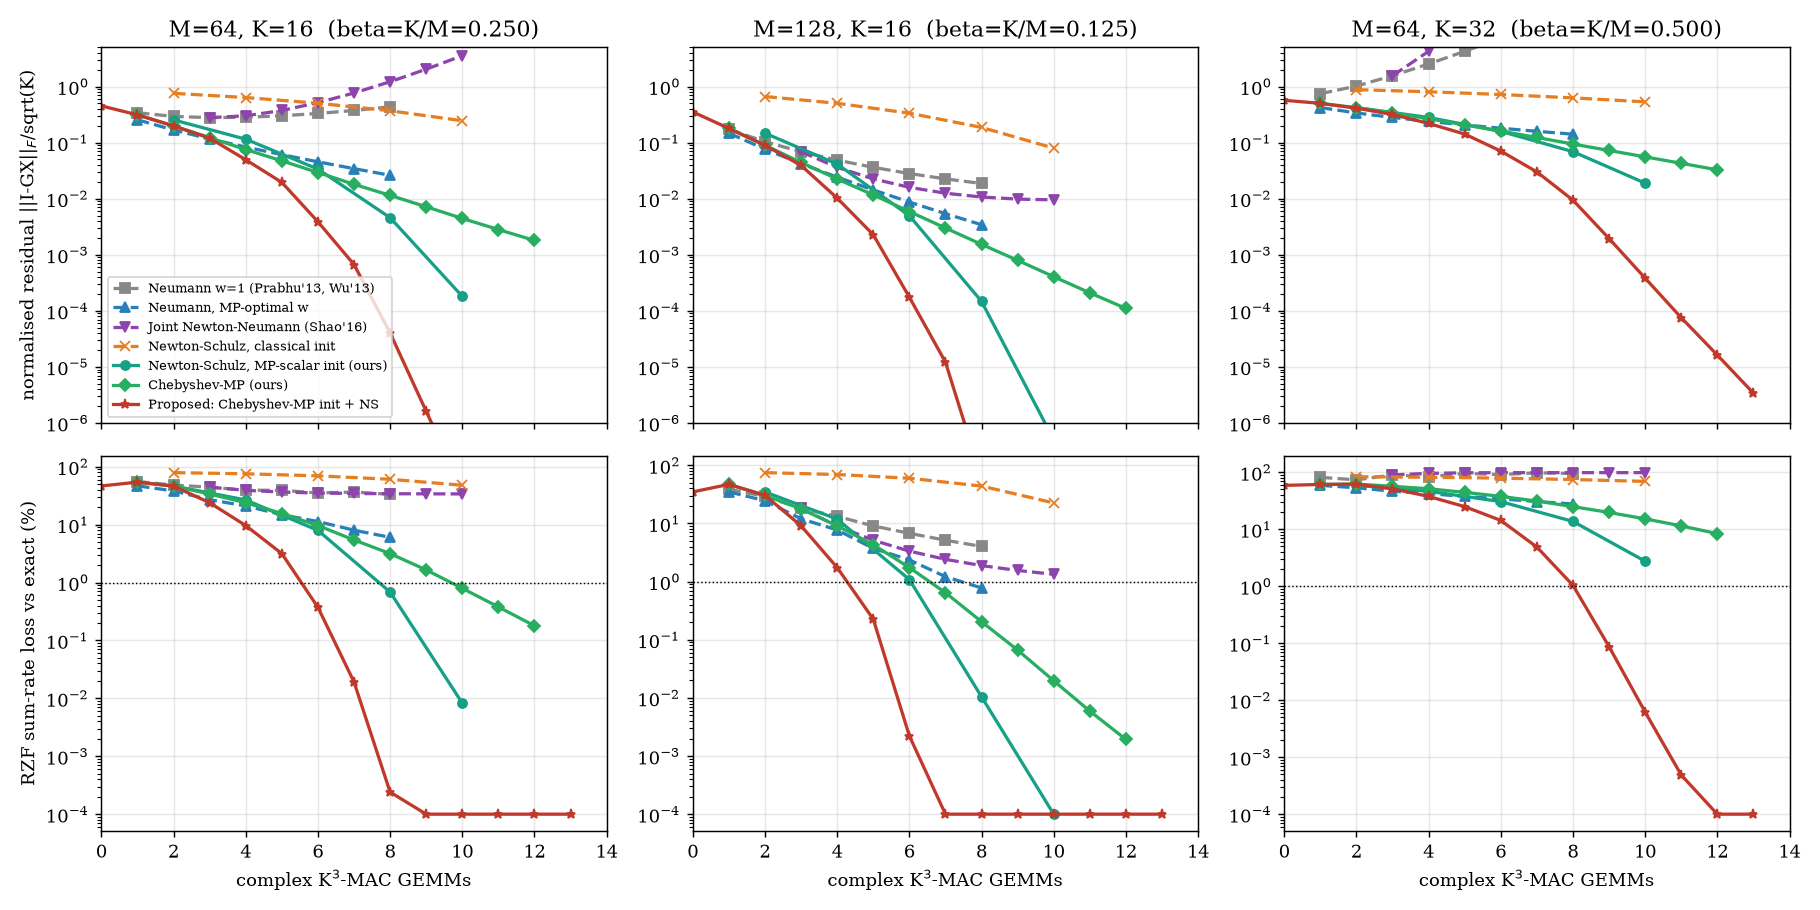
\includegraphics[width=\linewidth,height=0.72\textheight,keepaspectratio]{exp6_inversion_accuracy.png}
  \takeaway{Red curve (ours) reaches 1\,\% loss first in every antenna/user configuration.}
\end{frame}

\begin{frame}{Warm-start tracking across user speeds}
  \centering
  \small $K=16$, $M=64$; sum-rate loss vs exact RZF / GEMMs per slot per PRB\\[2mm]
  \begin{tabular}{lccc}
    \toprule
    Speed & Warm Gauss--Seidel $\times 4$ & Warm CG $\times 4$ & \textbf{RMT-WS (ours)} \\
    \midrule
    3 km/h & 0.009\,\% / 4 & 0.013\,\% / 5 & \best{0.006\,\% / 2.25} \\
    30 km/h & 0.63\,\% / 4 & 0.96\,\% / 5 & \best{0.43\,\% / 5.2} \\
    120 km/h & 2.9\,\% / 4 & 5.5\,\% / 5 & \best{0.12\,\% / 6.25} \\
    \bottomrule
  \end{tabular}
  \vspace{3mm}
  \begin{itemize}
    \item 3 km/h: \gd{2.7$\times$ fewer GEMMs} and \gd{30$\times$ lower loss} than a cold start
    \item 30 km/h: lowest loss of all warm-started methods
    \item 120 km/h: \gd{24$\times$ lower loss} than warm Gauss--Seidel
    \item Fixed 1- or 2-step warm starts diverge at 120 km/h --- RMT-WS never does
  \end{itemize}
  \takeaway{One method, every speed: cheap when users are slow, safe when they are fast.}
\end{frame}

\begin{frame}{Tracking: accuracy vs cost at 3, 30 and 120 km/h}
  \centering
  \vfill
  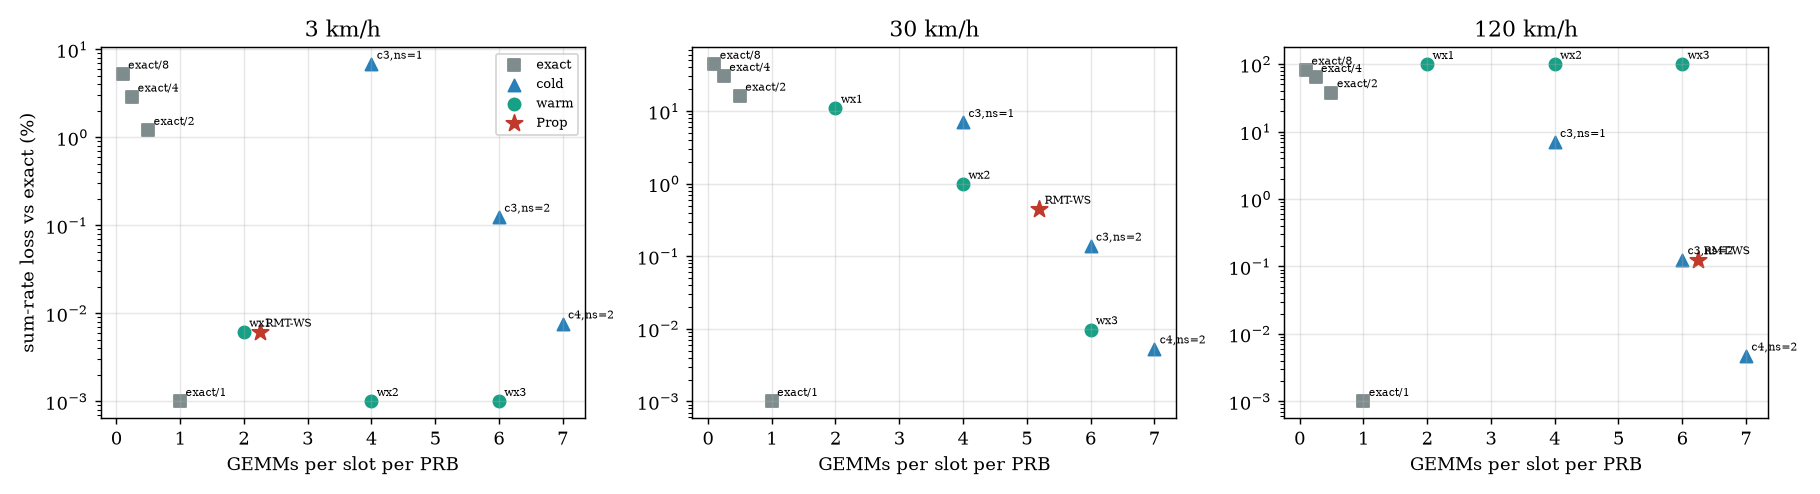
\includegraphics[width=\linewidth]{exp7_tracking.png}
  \takeaway{RMT-WS (red star) sits at the low-cost, low-loss corner at every speed.}
\end{frame}

\begin{frame}{A closed-form speed law and a safety certificate}
  \begin{columns}[c]
    \begin{column}{0.54\textwidth}
      \footnotesize
      \begin{block}{Doppler-to-warm-start law}
        \[ r_0 \approx c \cdot 2\sqrt{\tfrac{K}{M-K}}\,\sqrt{1-\rho}, \qquad 1-\rho \approx (\pi f_D T)^2 \]
        \begin{itemize}\footnotesize
          \item $r_0$ grows linearly with speed (measured slope 1.00)
          \item Predicts the Newton steps: $\lceil \log_2(\ln\varepsilon / \ln r_0) \rceil$
          \item Warm start valid up to $\approx$ \gd{39 km/h} (64/16), 60 km/h ($K=8$), 23 km/h ($K=32$)
        \end{itemize}
      \end{block}
      \begin{exampleblock}{Certified safety}
        \footnotesize
        Tail bound $\Pr(\hat r^2 \le (1-d) r^2) \le e^{-p d^2 s/2}$\\
        Audit of 480 PRB cases, 3--120 km/h: \gd{0} accepted-but-non-contractive at $\hat r \le 0.3$
      \end{exampleblock}
    \end{column}
    \begin{column}{0.42\textwidth}
      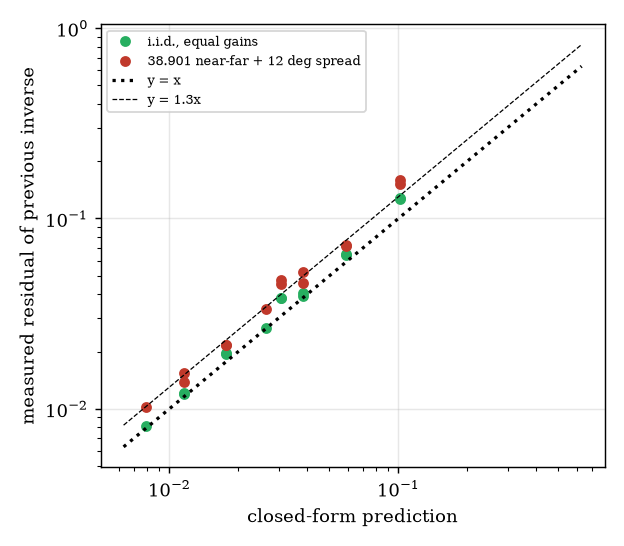
\includegraphics[width=\linewidth,height=0.62\textheight,keepaspectratio]{exp12_doppler_law.png}
    \end{column}
  \end{columns}
  \takeaway{A design rule: the DU knows in advance up to which speed the warm start pays off.}
\end{frame}

\begin{frame}{Robust at low precision}
  \centering
  \small GEMM operands rounded to $b$ mantissa bits, wide accumulate (tensor-core / NPU style)\\[2mm]
  \begin{columns}[c]
    \begin{column}{0.56\textwidth}
      \centering\footnotesize\setlength{\tabcolsep}{4pt}
      \begin{tabular}{lcc}
        \toprule
        Setting & Direct G--J & \textbf{Ours (Cheb + 3 NS)} \\
        \midrule
        8 mantissa bits & 0.88\,\% & \best{0.15\,\%} \\
        6 mantissa bits & 5.1\,\% & \best{1.4\,\%} \\
        Ill-cond., 10 bits & 1.2\,\% & \best{0.49\,\%} \\
        \bottomrule
      \end{tabular}
    \end{column}
    \begin{column}{0.4\textwidth}
      \begin{itemize}\footnotesize
        \item Sum-rate loss vs float64 exact
        \item \gd{6$\times$} lower loss at 8 bits, \gd{3.6$\times$} at 6 bits
        \item Newton iteration self-corrects rounding errors
        \item Tracker at 8 bits: 0.70\,\% vs 0.54\,\% at full precision (30 km/h)
      \end{itemize}
    \end{column}
  \end{columns}
  \takeaway{Our method is ready for low-precision accelerators where direct inversion degrades.}
\end{frame}

\begin{frame}{Low precision: loss vs mantissa bits}
  \centering
  \vfill
  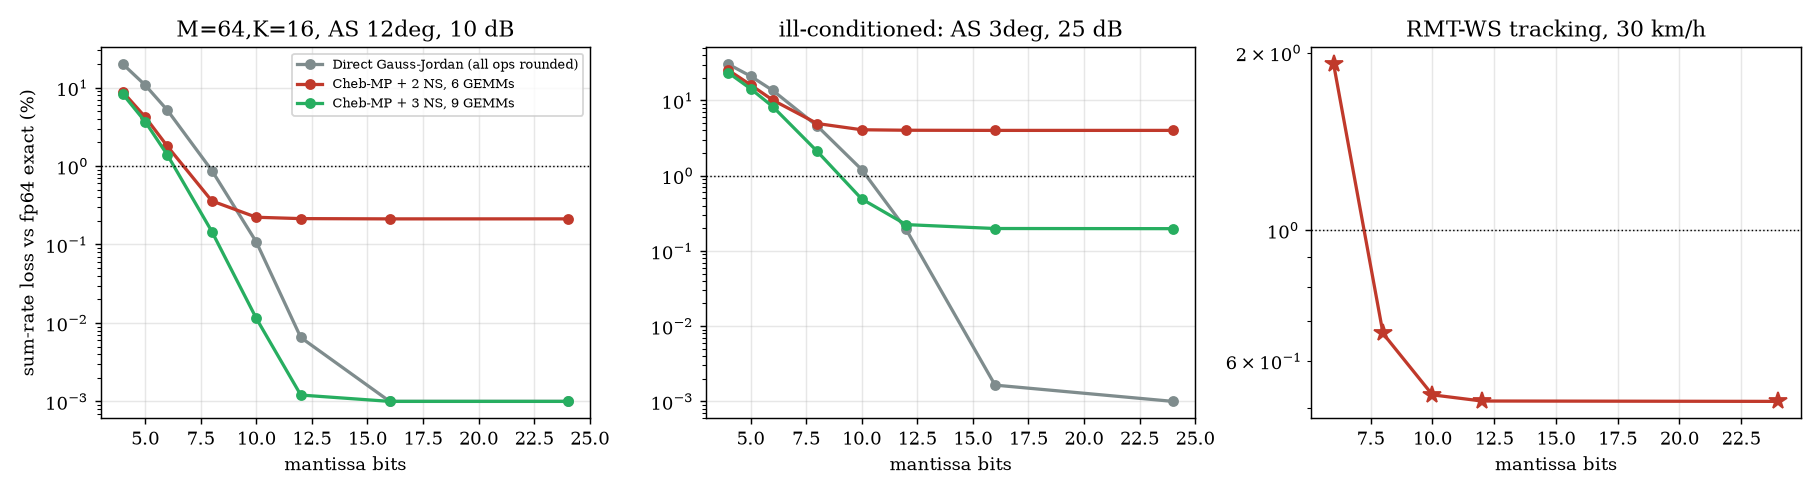
\includegraphics[width=\linewidth,height=0.7\textheight,keepaspectratio]{exp8_low_precision.png}
  \takeaway{Newton refinement keeps the loss low where direct inversion degrades.}
\end{frame}

% =====================================================================
\section{Kernel Programming}

\begin{frame}[fragile]{Kernel programming: a fused complex RZF precoder in C}
  \footnotesize \texttt{kernels/cmat\_kernels.c} --- batched complex64, AVX-512, OpenMP; binding \texttt{cmatinv/fastkernels.py}
  \begin{columns}[T]
    \begin{column}{0.54\textwidth}
      \begin{itemize}\footnotesize\setlength{\itemsep}{0pt}
        \item One pass per PRB: load $H$ once $\to$ Gram $\to$ inverse $\to$ $W^T$ + power scaling;
          stack / L1-resident, no DRAM intermediates
        \item Hermitian symmetry: Gram on the lower triangle only
        \item Split re/im planes so complex arithmetic vectorises
        \item In-place Gauss--Jordan sweep: $K$ rank-1 updates, no sqrt/divide chains
          (inverse 6.4k $\to$ \gd{2.9k} cycles/PRB, $K=16$)
        \item Register-blocked $W = H^H X$: 0.81 $\to$ \gd{0.42} ms/slot
        \item AVX-512 codegen: 1.3--1.5$\times$ single thread, 2$\times$ on 4 threads
        \item Fused Newton step returns the exact residual for free
      \end{itemize}
    \end{column}
    \begin{column}{0.44\textwidth}
\begin{lstlisting}
// inner loop of the sweep inverse
for (int i = 0; i < K; i++) {
  if (i == k) continue;
  float fr = ckr[i]*piv, fi = cki[i]*piv;
  float *ar = xr + i*K, *ai = xi + i*K;
  #pragma omp simd
  for (int j = 0; j < K; j++) {
    ar[j] -= fr*rkr[j] - fi*rki[j];
    ai[j] -= fr*rki[j] + fi*rkr[j];
  }
  ar[k] = -fr; ai[k] = -fi;
}

gcc -O3 -march=native -fopenmp
    -mprefer-vector-width=512
\end{lstlisting}
    \end{column}
  \end{columns}
\end{frame}

\begin{frame}{Kernel results: the whole precoder now fits in the slot}
  \centering
  \small 273 PRBs, complex64, 4-core AVX-512 Xeon, median of 40 runs\\[2mm]
  \begin{columns}[c]
    \begin{column}{0.55\textwidth}
      \centering
      \begin{tabular}{lccc}
        \toprule
        $K, M$ & numpy+LAPACK & \textbf{Our kernel} & Speed-up \\
        \midrule
        8, 64 & 1.08 ms & 0.070 ms & 15$\times$ \\
        \ours 16, 64 & 3.21 ms & \best{0.226 ms} & \best{14$\times$} \\
        32, 64 & 12.2 ms & 0.97 ms & 12.5$\times$ \\
        16, 128 & 4.71 ms & 0.41 ms & 11.6$\times$ \\
        32, 128 & 16.3 ms & 1.60 ms & 10$\times$ \\
        \bottomrule
      \end{tabular}
    \end{column}
    \begin{column}{0.42\textwidth}
      \begin{itemize}\small
        \item $K = 8, 16$ ($M=64$) and $K=16$, $M=128$ fit a 0.5 ms slot
        \item Near-linear thread scaling: 0.92 $\to$ 0.45 $\to$ 0.23 ms
        \item Accuracy: sum-rate loss $< 10^{-5}\,\%$ vs float64
      \end{itemize}
    \end{column}
  \end{columns}
  \takeaway{10--15$\times$ faster: from 6$\times$ over the slot budget to under half of it.}
\end{frame}

\begin{frame}{Whole-precoder time per slot (273 PRBs)}
  \centering
  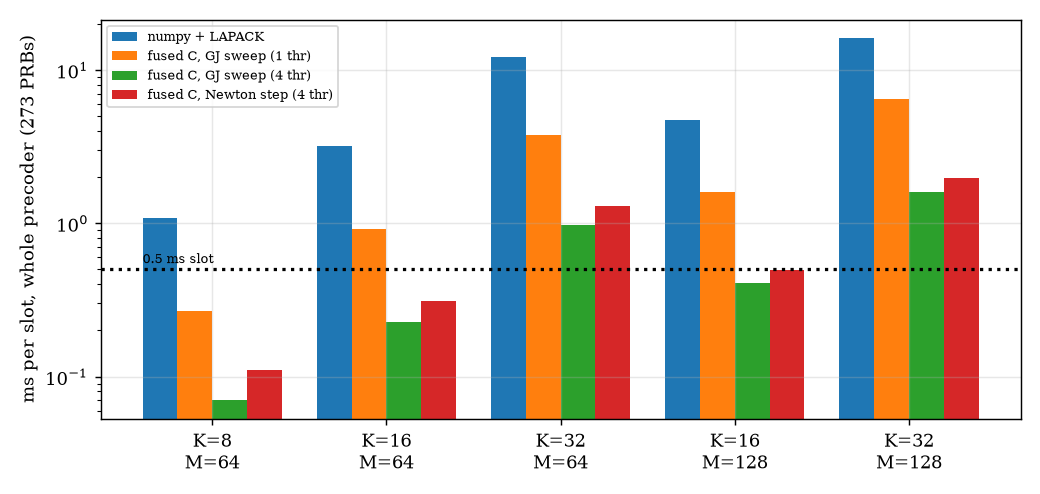
\includegraphics[width=\linewidth,height=0.7\textheight,keepaspectratio]{exp17_pipeline_kernel.png}
  \takeaway{Our fused kernels (green, red) run under the 0.5 ms line for $K \le 16$; numpy+LAPACK never does.}
\end{frame}

% =====================================================================
\section{Fronthaul Impact and Summary}

\begin{frame}{Where should precoding run? A 72\,\% fronthaul saving}
  \centering
  \small 100 MHz, $M=64$, $K=16$, BFP-9 IQ\\[2mm]
  \begin{tabular}{lcc}
    \toprule
    Architecture & Fronthaul & Sum-rate vs exact \\
    \midrule
    DU precodes, sends 64 streams & 118.4 Gbit/s & 100\,\% \\
    \ours RU precodes, 16 layers + 8-bit weights & \best{32.8 Gbit/s ($-72\,\%$)} & \best{99.7\,\%} \\
    RU precodes, 16 layers + 6-bit weights & 32.0 Gbit/s ($-73\,\%$) & 96.7\,\% \\
    \bottomrule
  \end{tabular}
  \vspace{3mm}
  \raggedright
  \begin{itemize}
    \item Mobility requires refreshing the weights every slot (every 4 slots: only 70\,\% of the rate at 30 km/h)
    \item Per-slot weights are exactly what our fast kernel delivers
    \item RU-side precoding cuts the link load by \gd{3.6$\times$}
  \end{itemize}
  \takeaway{Fast per-slot precoding unlocks a 72\,\% lighter fronthaul at 99.7\,\% of the rate.}
\end{frame}

\begin{frame}{Fronthaul rate and sum-rate by architecture}
  \centering
  \vfill
  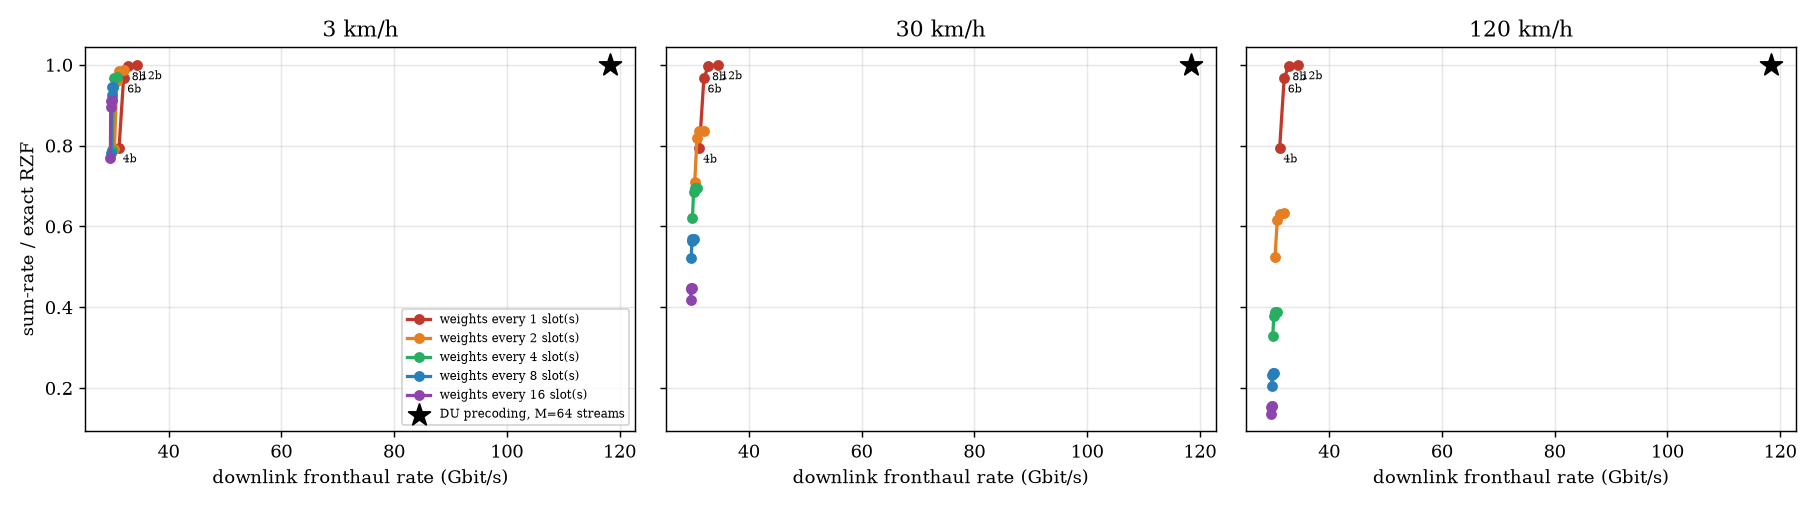
\includegraphics[width=\linewidth,height=0.7\textheight,keepaspectratio]{exp10_fronthaul.png}
  \takeaway{RU-side precoding with per-slot weights: $-72\,\%$ fronthaul at 99.7\,\% rate.}
\end{frame}

\begin{frame}{Part A summary}
  \centering
  \small
  \begin{tabular}{>{\raggedright}p{0.3\textwidth}p{0.62\textwidth}}
    \toprule
    Contribution & Headline result \\
    \midrule
    CSEE / RAS-BFP compression & 13--16$\times$ vs $\approx 4\times$ for O-RAN BFP; 3--6$\times$ faster than SVD; provable error bounds \\
    ACAFS adaptive split & 55--75\,\% bandwidth saving at high SNR \\
    RMT-WS cold start & 6 GEMMs vs $>10$ for Neumann / Newton-type; best at $K/M = 0.5$ \\
    RMT-WS tracking & 2.7$\times$ fewer GEMMs, 30$\times$ lower loss at 3 km/h; safe up to 120 km/h \\
    Speed law + certificate & Closed-form warm-start envelope; 0 unsafe decisions in 480 cases \\
    Low precision & 6$\times$ lower loss than direct inversion at 8 bits \\
    Fused C/AVX-512 precoder & 10--15$\times$ faster than numpy+LAPACK; $K \le 16$ fits the 0.5 ms slot \\
    RU-side precoding & $-72\,\%$ fronthaul at 99.7\,\% of exact sum-rate \\
    \bottomrule
  \end{tabular}
  \takeaway{Part A delivers a lighter link and a slot-feasible precoder --- the foundation for Part B.}
\end{frame}

\begin{frame}{Next: taking RMT-WS to GPU and tensor cores}
  \begin{itemize}
    \item RMT-WS is pure matrix multiplication --- the native operation of GPUs, NPUs and tensor cores
    \item $K = 16$ Gram matrices match a $16\times16$ tensor-core tile exactly
    \item Our low-precision results show the method keeps its accuracy at 8 bits
    \item Plan: CUDA port of the fused precoder; benchmark against cuBLAS / cuSOLVER batched
    \item Near-RT RIC deployment of ACAFS as an xApp
    \item Compression width as a per-cell knob for the Part B allocation rule
  \end{itemize}
  \vfill
  \centering
  {\Large\textbf{Thank you --- questions?}}
  \vfill
\end{frame}

\end{document}
